\documentclass[parskip=full]{uvamscse}


\usepackage{listings}

\lstdefinelanguage{sdf}{%
  numbers=none,
  morekeywords={module,imports,exports,sorts,context,lexical,free,syntax,==,=,+,-,left,cons,prefer,avoid,bracket},
  columns=flexible,
  morestring=[b]",
  basicstyle=\footnotesize\mdseries,
  literate={->}{{\,\,$\to$\,\,}}1
}

\lstdefinelanguage{dcg}{%
  numbers=none,
  morekeywords={},
  morestring=[b]",
  basicstyle=\footnotesize\mdseries,
  columns=flexible,
}

\lstdefinelanguage{prolog},
  literate={:-}{{\,$\Leftarrow$\,\,}}1 {-->}{{$\to$\,}}1
}

\lstdefinestyle{mono}{
  basicstyle=\footnotesize\ttfamily
}

\lstset{%
  frame=none,
  xleftmargin=2pt,
  stepnumber=1,
  numbers=left,
  numbersep=7pt,
  numberstyle=\ttfamily\scriptsize\color[gray]{0.3},
  belowcaptionskip=\bigskipamount,
  captionpos=b,
%  escapeinside={*'}{'*},
  % language=fl,
  tabsize=2,
  emphstyle={\bf},
  stringstyle=\itshape,
  showspaces=false,
  keywordstyle=\bfseries\rmfamily,
  columns=flexible,
  basicstyle=\small\mdseries,
  showstringspaces=false,
}

\newcommand{\cmd}[1]{\texttt{$\backslash$#1}}

\title{Detecting Violations of CSS Code Conventions}
% \coverpic[100pt]{figures/terminal.png}
% \subtitle{}
% \date{Spring 2014}


\author{Boryana Goncharenko}
\authemail{boryana.goncharenko@gmail.com}
% \host{Grammarware, Inc., \url{http://grammarware.github.io}}

\abstract{    

This section summarises the content of the thesis for potential readers who do
not have time to read it whole, or for those undecided whether to read it at
all. Sum up the following aspects:

  \begin{itemize}
    \item relevance and motivation for the research
    \item research question(s) and a brief description of the research method
    \item results, contributions and conclusions
  \end{itemize}
}


\begin{document}
\maketitle

%%%%%%%%%%%%%%%%%%%%%%%%%%%%%%%%%%%%%%%%%%%%%%%%%%%%%%%%%%%%%%%%%%%%%%%%%%%%%%%%
\chapter{Introduction}

Code conventions put constraints on how code should be written in the context of a project,
organization or programming language. Style guides can comprise conventions that refer to
whitespacing, indentation, code layout, preference of syntactic structures, code patterns and anti-
patterns. They are mainly used to achieve code consistency, which in turn improves the readability,
understandability and maintainability of the code [Citations].

Style guides are often designed in an ad hoc manner. Coding conventions typically live in documents
that contain a description of each rule in natural language accompanied by code examples. This is
the case with the style guidelines of Mozilla [8], Google [6], GitHub [10], WordPress [11] and
Drupal [4]. To apply the conventions, developers first need to read, understand and apply them
manually. Such an approach introduces a number of issues. Using natural language can make guidelines
incorrect, ambiguous, implicit or too general. Another problem is that developers apply conventions
manually, which increases the chances of introducing violations involuntarily. There are tools that
check for compliance with guidelines, however, they are often hard to customize or limited to one
type of violations, e.g. only whitespacing.

The core idea behind the project is to provide a solution that lets developers express an arbitrary
set of coding conventions and detect their violations automatically in an IDE. Writing conventions
in an executable form could assist authors in detecting incorrect, ambiguous or inconsistent
guidelines. Automatic detection of violations could minimize the effort required by developers to
write code that complies to the guidelines. To meet the constraints of a Master’s project, the
implementation is limited to the domain of Cascading Style Sheets (CSS). The project requires
determining the need for CSS code conventions in organizations, collecting and analyzing available
style guides, and providing a way to express conventions. Specifically, the project attempts to
answer the following set of questions:

  \begin{itemize}
    \item \textbf{Research Question 1:} Do developers still maintain plain CSS?
    \item \textbf{Research Question 2:} What code conventions for CSS exist?
    \item \textbf{Research Question 3:} How to express existing CSS code conventions?
  \end{itemize}

The thesis is organized as follows. Chapter 2 contains background notions and terms used throughout
the thesis. The method and results for RQ1 are presented in Chapter 3. Discovering the existing code
conventions is illustrates in Chapter 4. The design and description of a DSL is presented in Chapter
5. Chapter 6 concludes the thesis.



%%%%%%%%%%%%%%%%%%%%%%%%%%%%%%%%%%%%%%%%%%%%%%%%%%%%%%%%%%%%%%%%%%%%%%%%%%%%%%%
\chapter{Background}

\section{Bunge-Wand-Weber ontology}

A \textbf{conceptualization} is an abstract, simplified view of the world that is represented for
some purpose~\cite{gruber1995toward}. It consists of the concepts that are assumed to exist in some
area of interest and their relationships~\cite{gruber1995toward}. An \textbf{ontology} is an
explicit specification of a conceptualization~\cite{gruber1995toward}. It describes what is
fundamental in the totality of what exists and it defines the most general categories to which we
need to refer in constructing a description of reality~\cite{milton2004top}.

Milton further distinguishes between two kinds of ontologies: top-level and domain-
specific~\cite{milton2004top}. Ontologies of the former type are highly general and provide the
theoretical foundations for representation and modeling of systems. Ontologies of the latter type
are restricted to define concepts and their relations that fall in a particular domain. Every
domain-specific ontology needs to use categories that are captured in a top-level ontology. In this
sense a domain-specific ontology is based on a specific top-level ontology~\cite{milton2004top}.

The Bunge-Wand-Weber (BWW) ontology~\cite{wand1990ontological} is a high-level ontology used in the representation model developed by Wand and Weber~\cite{wand1995deep}. Table 2.1 presents a selected set of the ontological constructs in the BWW ontology.

\begin{center}
\begin{longtable}{ | p{11em} | p{30em} | } 
\caption{Selected ontological constructs in the BWW representation model}\\
\hline
 &  \\
\textbf{Ontological construct} & \textbf{Explanation} \\
 &  \\
\hline
Thing & The elementary unit in the BWW ontological model. The real world is made up of things. A composite thing may be made up of other things (composite or primitive). \\ 
\hline
Properties & \multirow{7}{30em}{Things possess properties. A property is modeled via a function that maps the thing into some value. A property of a composite thing that belongs to a component thing is called an hereditary property. Otherwise it is called an emergent property. A property that is inherently a property of an individual thing is called an intrinsic property. A property that is meaningful only in the context of two or mode things is called a mutual or relational property.} \\ 
 &  \\ 
 &  \\
 &  \\
 &  \\
 &  \\
 &  \\
 \hline
 State & A vector of values for all property functions of a thing. \\
 \hline
 Event & A change of state of a thing. It is effected via a transformation. \\
 \hline
 Transformation & A mapping from a domain comprising states to a codomain comprising states. \\
 \hline
 History & The chronologically ordered states that a thing traverses. \\
 \hline
 Coupling & A thing acts on another thing if its existence affects the history of the other thing. The two things are said to be coupled or interact. \\
 \hline
 Class & A class is a set of things that can be defined via their possessing a characteristic property. \\ 
 \hline
 Kind & A kind is a set of things that can be defined only via their possessing two or more properties. \\ 
\hline
 System & A set of things is a system if, for any bi-partitioning of the set, couplings exist among things in the two subsets. \\
 \hline
 System Composition & The things in the system are its composition. \\
 \hline
 System Environment &  Things that are not in the system but interact with things in the system are called the environment of the system. \\
 \hline
\end{longtable}
\end{center}


\section{Ontological analysis}

\textbf{Ontological analysis} is an established approach for evaluating the quality of software engineering notations~\cite{moody2009physics}. It consists of a two way comparison between a set of modeling grammar constructs and a set of ontological constructs. The \textbf{interpretation mapping} compares the notation with the ontology and the \textbf{representation mapping} compares the ontology with the notation~\cite{gehlert2007toward}. The underpinning of ontological analysis is that modeling grammars are incomplete if they are not able to represent what exists in reality~\cite{green2000integrated}. Furthermore, the analysis requires one-to-one mapping between the modeling grammar and the ontological constructs. Any deviation from such correspondence leads to an anomaly (Figure 2.1).

\begin{figure}[h!]
  \centering
  \caption{Ontological Analysis~\cite{gehlert2007toward}}
  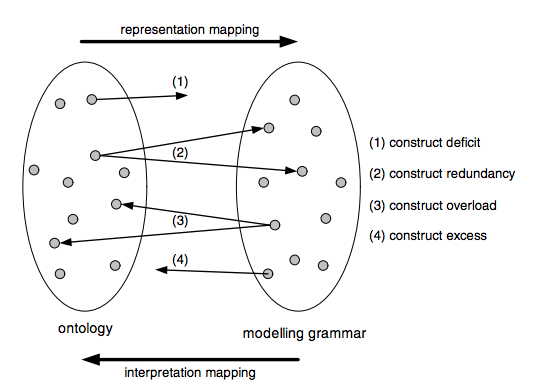
\includegraphics[width=0.65\textwidth]{ontoanalysis}
\end{figure}

\textbf{Construct deficit} occurs when an ontological construct does not have a corresponding construct in the modeling grammar. \textbf{Construct redundancy} is observed when a single ontological construct maps to more than one modeling grammar construct. \textbf{Construct overload} appears when a modeling grammar construct corresponds to more than one ontological construct. \textbf{Construct excess} occurs when a modeling grammar construct does not map to any ontological construct.~\cite{moody2009physics}

%%%%%%%%%%%%%%%%%%%%%%%%%%%%%%%%%%%%%%%%%%%%%%%%%%%%%%%%%%%%%%%%%%%%%%%%%%%%%%%
\chapter{Evaluating the Need for CSS Code Conventions}

I will talk about answering the first research question.

\section{Research Method}

Despite the new features added in the second~\cite{CSS2} and third~\cite{CSS3} versions of CSS, the
language has obvious limitations, for example, lack of variables. A number of preprocessors have
evolved to tackle the downsides of CSS. Solutions such as SASS~\cite{SASS}, LESS~\cite{LESS} and
Stylus~\cite{Stylus} offer enhanced or even different syntax and translate it to CSS. Preprocessors
are not only ubiquitously recommended, but also widely adopted in practice. The presence of such
solutions poses the question whether conventions for CSS are required at all. If nowadays CSS is
generated and not handcrafted, there is not need for conventions for CSS. There is need for
conventions for the preprocessor languages.

To determine whether CSS is still handcrafted, all commits to open source repositories hosted on
GitHub for the period Jan-Apr 2015 have been analyzed. To differentiate between plain CSS and
preprocessor code, the extensions of all files in the commits were inspected. In case the commit
contains a file with extension \texttt{.scss}, \texttt{.sass}, \texttt{.less} or \texttt{.styl}, it
is considered preprocessor maintenance. In case the commit contains files with the \texttt{.css}
extension and no preprocessor extensions, it is considered maintenance of plain CSS. Since the main
objective of the search is to determine maintenance, only files that were modified are taken into
consideration. Files that were added are excluded from the results, since developers often add
third-party CSS libraries to their repositories.

\section{Results}

A total of X repositories and X commits have been analyzed. The number of commits that maintain any form of CSS is X. Almost 60 percent of these commits still show plain CSS. 
Despite of the popular belief that nowadays preprocessors are prevailing than CSS, results
illustrate plain CSS is still used. Figure 1 summarizes the findings.

Having the above in mind I assume that CSS is still maintained in practice.

\section{Analysis}

What if the main users of preprocessors are private?

What if the time interval was too short?

What if there are other preprocessor that are not counted?

%%%%%%%%%%%%%%%%%%%%%%%%%%%%%%%%%%%%%%%%%%%%%%%%%%%%%%%%%%%%%%%%%%%%%%%%%%%%%%%

\chapter{Discovering Existing CSS Code Conventions}

\section{Research Method}

The CSS community has produced a pool of recommendations, best practices, and style guides, but how
to choose the among them? Since the primary organization responsible for the specification of CSS
has not recommended code conventions, any selection strategy based on the author of the conventions
could be considered cherry picking.

To determine the set of code conventions, two searches with the keywords “CSS code conventions” have
been made using the search engines http://duckduckgo.com and http://google.com. The first 50 results
of each search have been analyzed. From each result only conventions about pure CSS are taken into
account and guidelines for CSS preprocessors are ignored. In case the result is an online magazine
or a blog post that links to other resources, these references are considered as results and
analyzed separately.

Discuss problem with conventions here: 
\begin{description}

\item Overgeneralized conventions - The description of the convention is too general to be applied,
e.g. ``don’t use CSS hacks — try a different approach first''.

\item Incorrect conventions - There is a discrepancy between the description of the rule and the
provided example. An instance of such contradiction is when the convention ‘nothing but declarations
should be indented’ is followed by a code snippet illustrating that rules in media queries should
also be indented.

\item Ambiguous conventions - There is more than one interpretation of a convention. For example,
‘rules with more than 4 selectors are not allowed’ could be seen as forbidding multi- selectors with
more than four selectors, or disallowing selectors with more than four simple- selectors.

\item Implicit conventions - There are rules that are not explicitly stated and could only be
inferred by the other rules. For example, the convention ‘you can put values on multiple lines’ is
not preceded by a convention that requires values to appear on one line.

\item Inconsistencies between conventions in one ruleset - Google say that charsets should not be
used in css, but later say that in charsets double quotes should be used. Surely, this opens the
question - so when do I need to use charsets? 

\end{description}

\section{Results}

Results of the two searches include the CSS coding guidelines of CSS professionals as well as
leading companies, e.g. Google, Mozilla, GitHub, Wordpress. The accumulated corpus consists of 165
unique coding conventions. . Here is an example:

A full list is available at this GitHub page.

\section{Analysis}

There are conventions that cannot be detected at all?

What if not everyone have published their style guides? Well, some respectful companies did.

%%%%%%%%%%%%%%%%%%%%%%%%%%%%%%%%%%%%%%%%%%%%%%%%%%%%%%%%%%%%%%%%%%%%%%%%%%%%%%%

\chapter{Expressing CSS Code Conventions}

\section{Analysis of conventions corpus}

Code conventions is an umbrella term that comprises a vast set of rules. To check what the CSS
conventions are all about, I analyzed the conventions and it turned out there are three broad groups
of conventions. In general, CSS conventions refer to whitespacing and indentation, to syntax
preference or to programming style.

Further, the analysis consists of analyzing each individual convention.

The approach used to explore the domain consists of analyzing how the current system works. In other
words, the analysis aims at revealing how developers detect violations manually, what is knowledge
developers need and what are the particular steps they make. The domain analysis phase consists of
two steps:

  \begin{itemize}
    \item Determine possible violations. In this step the meaning of the convention is discussed and violations are made explicit.
    \item List the specific actions that need to be taken to detect violations manually. Developers check their code for compliance manually. To perform such checks, developers need to understand different concepts, e.g. the concept of a rule, html element, ids, etc and perform certain actions, such as find a structure, evaluate a constraint etc.
  \end{itemize}

The following analysis of three conventions illustrates the process described above. Analysis of all
conventions in the corpus are available at GitHub.

\begin{description}
\item \textbf{Convention:} Disallow empty rules.
\item \textbf{Author:} CSS lint
\item \textbf{Violations:} Presence of rulesets that do not contain declarations. In case at least one declaration is present, the ruleset does not violate the convention. Examples include:
\begin{sourcecode}
\begin{lstlisting}[style=mono,language=Java]
.myclass { }  /* violation */
.myclass { /* Comment */ } /* violation */
.myclass { color: green; } /* not violation */
\end{lstlisting}
\end{sourcecode}

\item \textbf{Actions:} Recognize rulesets and declarations. Determine whether a ruleset does not contain any declarations.

\end{description}

This convention aims at getting rid of one type of refactoring leftovers - rulesets without
declarations [CSS lint]. Removing empty rulesets reduces the total size of CSS that needs to be
processed by the browser. One possible approach for discovering violations of the convention at hand
is to search the stylesheet for rulesets and then check whether each ruleset contains a declaration.
To perform this search successfully, developers need to understand the concept of a ruleset and a
declaration, i.e. they need to be able to recognize these two CSS structures. Further, developers
need to determine relations between structures, particularly, whether a ruleset contains a
declaration.

In this way, all conventions have been analyzed and as a result, the following set of conclusions
have been made:

1) Every convention imposes a set of constraints over the program. Violations occur when these
constraints are not met.

2) Conventions can refer to nodes in abstract syntax tree, concrete syntax tree and parse tree of
CSS.

3) Conventions can refer to nodes based on their type or function in the program (hex, color)

4) Conventions can refer to nodes based on CSS-specific knowledge, e.g. is vendor-specific property

4) Conventions can refer to nodes based on their context. Typically, conventions do not target a
node in isolation but a number of related nodes that form a pattern. The nodes do not have to be
immediately related, they could be scattered across the tree.

5) Conventions could be related. For example, it is often the case that two conventions are related
within the boundaries of a style guide. Often a given convention serves as an exception for another
convention, or relaxes the constraints of another convention.


\section{Abstract syntax}

TODO: shall I add context and convention diagrams
Types are still missing

This section describes the abstract syntax of CssCoco. An overview of the abstract syntax is shows in Figure x. A detailed view of each of the .. is presented afterwards.

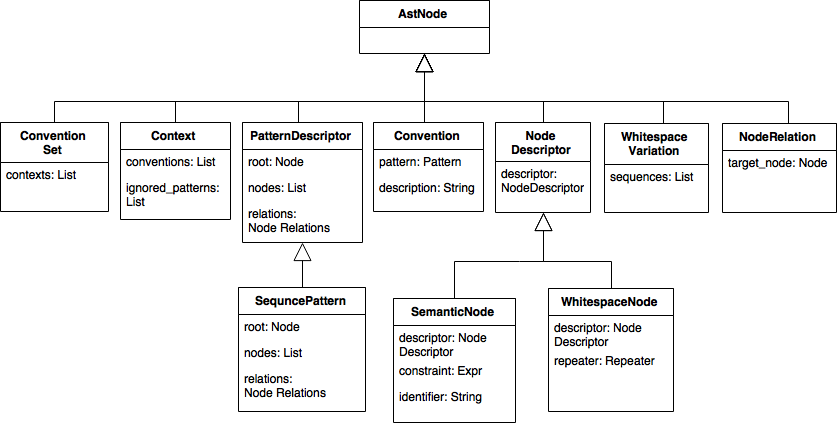
\includegraphics[width=\textwidth]{general}

\begin{description}

\item\textbf{ConventionSet} represents a style guide. It comprises a number of conventions that form coherent guidelines. Attribute \texttt{contexts} is a list of Contexts that contain conventions.


\item\textbf{Context} represents a group of conventions that belong to the same semantic group (e.g. whitespacing, syntax preference, programming style). Attribute \texttt{conventions} is a list of Contexts that contain conventions. Attribute \texttt{ignored\_patterns} is a list of Patterns that are ignored while searching for the target pattern. For example, while searching for violations of semantic conventions, the whitespacing and indentation nodes are ignored.


\item\textbf{Convention} represents a rule that enforces specific constraints. Attribute \texttt{pattern} is the pattern that the convention targets. Attribute \texttt{description} is the description of the convention in natural text. This description is displayed to the user when a violation of the convention is discovered.


\item\textbf{Pattern} represents a description of a node or a combination of related nodes that given convention constraints.  Attribute \texttt{root} is the top node described in the pattern. Attribute \texttt{nodes} is a collection of all nodes described by the pattern. Attribute \texttt{relations} is a collection of relationships between the nodes used in the pattern.


\item\textbf{SequencePattern} represents a special type pattern in which nodes are allowed to be only siblings. Attribute \texttt{root} is the top node described in the pattern. Attribute \texttt{nodes} is a collection of all nodes described by the pattern. Attribute \texttt{relations} is a collection of relationships between the nodes used in the pattern.


\item\textbf{Node} represents a description of a non-whitespace node used in a Pattern.  
Attribute \texttt{descriptor} contains information about the type of the described node. Attribute \texttt{constraint} is an expression that designates additional constraints applied to the node. Attribute \texttt{identifier} is a given string that can be used as a reference to the matched node.


\item\textbf{WhitespaceNode} represents a description of a whitespace node that references space, newline, indentation symbols. Attribute \texttt{descriptor} contains information about the type of the described node. Attribute \texttt{repeater} is an optional constraint that specific the number of times a whitespace node can appear consecutively. Repeaters are useful to express conventions that do not specify exact quantities of whitespace symbols. For example, the convention ``put at least one blank line between rules'' sets a lower limit of the number of blank lines, but not an upper limit.


\item\textbf{WhitespaceVariation} represents a description of acceptable whitespace sequences. Whitespace variations are allowed to appear as operands of BeforeExpr, AfterExpr and BetweenExpr.  Attribute \texttt{descriptor} contains information about the type of the described node. Attribute \texttt{constraint} is an expression that designates additional constraints applied to the node. Attribute \texttt{identifier} is a given string that can be used as a reference to the matched node.


\item\textbf{NodeDescriptor} represents a description of the type of the Node. Conventions refer to nodes using their CSS type, their function in the CSS program or their concrete syntax representation. For example, the code ``\#E6E6E6'' can be addressed both as a hexadecimal value and as a color. Attribute \texttt{func} is a lambda function that determines whether a node meets the type constraint. This function is used to select match candidates while searching the CSS tree for violation patterns. In this way the additional constraints imposed by the Node are evaluated only for the candidates.


\item\textbf{NodeRelation} represents a relation between two Nodes. Specializations of node relation are previous sibling, next sibling, parent and ancestor relations. Attribute \texttt{target\_node} designates the Node targeted by the relation.

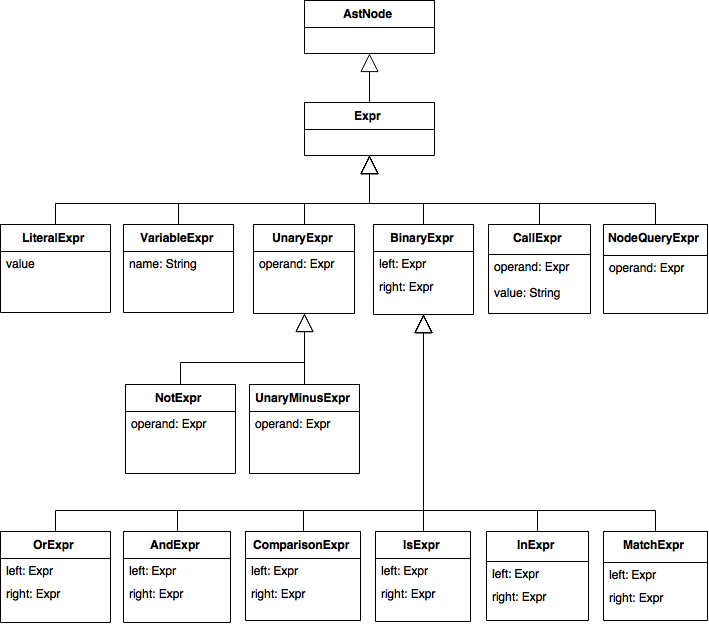
\includegraphics[width=\textwidth]{expr}

\item\textbf{LiteralExpr} represents an expression containing a literal value. Attribute \texttt{value} is the value of the literal expression.

\item\textbf{VariableExpr} represents a reference to a matched node. Attribute \texttt{name} is the identifier used to reference the node.

\item\textbf{UnaryExpr} represents expressions with a single operand. Attribute \texttt{operand} is operand of the expression.

\item\textbf{NotExpr} represents logical negation expression.

\item\textbf{UnaryMinusExpr} represents unary minus expression.

\item\textbf{BinaryExpr} represents expressions with a two operands.

Attributes \texttt{left} and \texttt{right} represent the first and second operands, respectively.

\item\textbf{OrExpr} represents logical disjunction expression.

\item\textbf{AndExpr} represents logical conjunction expression.

\item\textbf{ComparisonExpr} represents expression that compares two operands.

\item\textbf{IsExpr} represents expression that checks whether the first operand is of the given type, specified by the second operand.

\item\textbf{InExpr} represents expression that checks whether the first operand is present in a list of values, specified by the second operand.

\item\textbf{MatchExpr} represents expression that checks whether the first operand matches a regular expression, specified by the second operand.

\item\textbf{CallExpr} represents expression that invokes a API property or method of the operand. Attribute \texttt{operand} is the operand of the expression. Attribute \texttt{value} is the name of the API property or method that is invoked.

\item\textbf{NodeQueryExpr} represents expression that queries node context. Attribute \texttt{operand} is the node used as a reference point for the query.


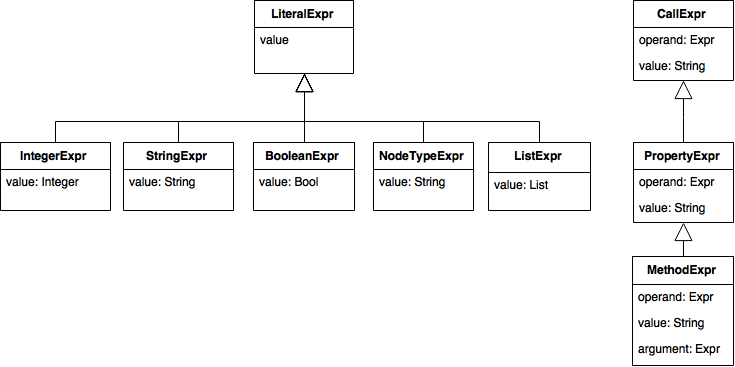
\includegraphics[width=0.9\textwidth]{literal}

\item\textbf{IntegerExpr} represents expression containing a integer value.

\item\textbf{StringExpr} represents expression containing a string value.

\item\textbf{BooleanExpr} represents expression containing a boolean value.

\item\textbf{ListExpr} represents expression containing a list value. The elements of the list are of type LiteralExpr.

\item\textbf{NodeTypeExpr} represents expression containing a string value that describes node type.

\item\textbf{PropertyExpr} represents an expression that returns the value of a property of the operand node. Attribute \texttt{operand} represents the node targeted by the expression. Attribute \texttt{value} holds the name of the property that is accessed.

\item\textbf{MethodExpr} represents an expression that returns invokes a method of the operand node. Attribute \texttt{argument} represents argument passed to the invoked method.

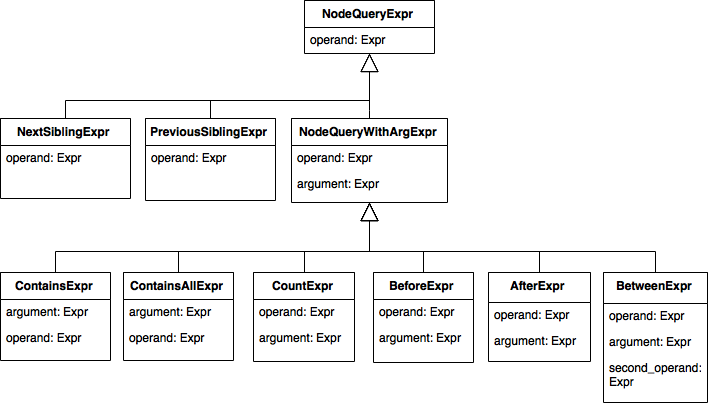
\includegraphics[width=0.9\textwidth]{nodequery}

\item\textbf{NextSiblingExpr} represents expression that returns the following sibling of the operand node.

\item\textbf{PreviousSiblingExpr} represents expression that returns the previous sibling of the operand node.

\item\textbf{NodeQueryWithArgExpr} represents expression that queries node context and uses additional constraints for the query. Attribute \texttt{argument} represents the additional constraints used by the query.

\item\textbf{ContainsExpr} represents an expression that checks whether the operand node contains a node that matches given constraints.

\item\textbf{ContainsAllExpr} represents an expression that checks whether the operand node contains nodes that match given constraints.

\item\textbf{CountExpr} represents an expression that counts the number of ancestor nodes of the operand that match a given constraint.

\item\textbf{BeforeExpr} represents an expression that checks whether a given whitespace variation appears before the operand node.

\item\textbf{AfterExpr} represents an expression that checks whether a given whitespace variation appears after the operand node.

\item\textbf{BetweenExpr} represents an expression that checks whether a given whitespace variation appears between the two operand nodes.

\end{description}

\section{Concrete syntax}

This section contains the concrete syntax of the designed DSL. Below are presented the grammar rules accompanied by the mapping to the abstract syntax of the language.


\begin{description}

\item\textbf{stylesheet} represents a style guide.

Abstract Syntax Mapping: ast.ConventionSet.

\begin{snippet}
\begin{verbatim}
stylesheet : context* ;
\end{verbatim}
\end{snippet}

\item\textbf{context} represents a group of logically related conventions. A single style guide can comprise a number of conventions that enforce various constraints, e.g. whitespacing, syntax preference, program style. Such categories refer to different types of nodes and require ignoring certain patterns.  

Abstract Syntax Mapping: ast.Context.

\begin{snippet}
\begin{verbatim}
context : Identifier '{' convention* '}' ;
\end{verbatim}
\end{snippet}

\item\textbf{convention} represents a single rule in the style guide. Conventions are typically expressed by directly stating what is disallowed or describing a condition that if met, requires additional constraints. The former way of expressing conventions are represented by the \texttt{forbid} conventions. The latter approach uses the structure \texttt{find ... require ...}. To break down complex disallowing conventions, the structure \texttt{find ... forbid ...} has been introduced. It aims at improving readability of conventions. 

Abstract Syntax Mapping: ast.Convention.

\begin{snippet}
\begin{verbatim}
convention : 'forbid' pattern 'message' String
           | 'find' pattern ('require'|'forbid') logic_expr 'message' String
           ;
\end{verbatim}
\end{snippet}

\item\textbf{pattern} represents a pattern of nodes and their relations. It can describe a horizontal sequence of sibling nodes and or a vertical pattern of nested nodes. Also, it can describe pairs of elements. 

Abstract Syntax Mapping: ast.Pattern.

\begin{snippet}
\begin{verbatim}
pattern : node_declaration (('in'|'next-to') node_declaration)*
        | fork ('in' node_declaration)*
        ;
fork : '(' node_declaration (',' node_declaration)+ ')' ;
node_declaration : (Identifier '=')? semantic_node ;
\end{verbatim}
\end{snippet}

\item\textbf{semantic\_node} represents a non-whitespace node. It describes the type of the node and its additional constraints. 

Abstract Syntax Mapping: ast.Node.

\begin{snippet}
\begin{verbatim}
semantic_node : node_type ('{' logic_expr '}')? ;
\end{verbatim}
\end{snippet}

\item\textbf{whitespace\_variation} represents a sequence of whitespace nodes. They differ from the rest of the nodes types because the user can specify how many times they need to be consecutively repeated. 

Abstract Syntax Mapping: ast.WhitespaceVariation, ast.WhitespaceNode, ast.Repeater.

\begin{snippet}
\begin{verbatim}
whitespace_variation : whitespace_node ('or' whitespace_node)* ;
whitespace_node : Identifier ('{' repeater '}')? ;
repeater : Integer ',' Integer? | (',')? Integer ;
\end{verbatim}
\end{snippet}

\item\textbf{logic\_expr} represents expressions that perform logic operations and glue arithmetic and type expressions. 

Abstract Syntax Mapping: ast.NotExpr, ast.AndExpr, ast.OrExpr and all arithmetic\_expression and type\_expression mappings.

\begin{snippet}
\begin{verbatim}
logic_expr : '(' logic_expr ')'
           | 'not' logic_expr
           | logic_expr 'and' logic_expr
           | logic_expr 'or' logic_expr
           | type_expr
           | arithmetic_expr
           ;
\end{verbatim}
\end{snippet}

\item\textbf{type\_expr} represents expressions that ensure node type and perform node queries of whitespace nodes. They are located in a separate parser rule because they interpret Identifiers as node type expressions instead of a API calls. 

Abstract Syntax Mapping: ast.IsExpr, ast.BeforeExpr, ast.AfterExpr, ast.BetweenExpr.

\begin{snippet}
\begin{verbatim}
type_expr : arithmetic_expr operator='is' type_=Identifier
          | whitespace_variation ('before' | 'after') type_operand
          | whitespace_variation 'between' type_operand 'and' type_operand
          ;
type_operand : Identifier | semantic_node ;
\end{verbatim}
\end{snippet}

\item\textbf{arithmetic\_expr} represents arithmetic, comparison, set membership and regex expressions. These are located in a separate parser rule because they interpret identifiers as API calls instead of node type expressions.

Abstract Syntax Mapping: ast.UnaryMinus, ast.UnaryPlus, ast.LessThan, ast.LessThanOrEq, ast.GreaterThan, ast.GreaterThanOrEq, ast.Equal, ast.NotEqual, ast.InExpr, ast.MatchExpr, ast.LiteralExpr.

\begin{snippet}
\begin{verbatim}
arithmetic_expr : ('-'|'+') arithmetic_expr
                | arithmetic_expr ('<'|'>'|'<='|'>='|'=='|'!=') arithmetic_expr
                | arithmetic_expr ('in'|'not in'|'match'|'not match') arithmetic_expr
                | call_expression
                | element
                ;
element : Boolean | Integer | String | list_ ;
\end{verbatim}
\end{snippet}

\item\textbf{call\_expr} represents an API call expression and also node query expression.

Abstract Syntax Mapping: ast.CallExpr and ast.NodeQueryExpr.

\begin{snippet}
\begin{verbatim}
call_expr : call_expr '.' call_expr
          | Identifier ('(' (element | semantic_node ) ')')? 
          ;
\end{verbatim}
\end{snippet}

\item\textbf{Boolean:} represents Boolean literal expression. 

Abstract Syntax Mapping: ast.BooleanExpr.

\begin{snippet}
\begin{verbatim}
Boolean : 'true' | 'True' | 'false' | 'False' ;
\end{verbatim}
\end{snippet}

\item\textbf{String:} represents String literal expression.

Abstract Syntax Mapping: ast.StringExpr.

\begin{snippet}
\begin{verbatim}
String : "'" (EscapeSequence | ~['])*? "'" ;
EscapeSequence : "\\" "'" ;
\end{verbatim}
\end{snippet}

\item\textbf{Integer:} represents Integer literal expression. 

Abstract Syntax Mapping: ast.IntegerExpr.

\begin{snippet}
\begin{verbatim}
Integer : (ZeroDigit | NonZeroDigit Digit*) ;
Digit : ZeroDigit | NonZeroDigit ;
NonZeroDigit : [1-9] ;
ZeroDigit : [0] ;
\end{verbatim}
\end{snippet}

\item\textbf{list} and \textbf{list\_element} represent the List literal expression. 

Abstract Syntax Mapping: ast.ListExpr.

\begin{snippet}
\begin{verbatim}
list_ : '[' list_element (',' list_element)* ']' ;
list_element : Integer | String | semantic_node ;
Letter : [a-zA-Z] ;
Identifier : (Letter)(Letter|Digit|'_'|'-')* ;
\end{verbatim}
\end{snippet}

\item\textbf{type\_expression} represents the NodeType literal expression.

Abstract Syntax Mapping: ast.NodeType.

\begin{snippet}
\begin{verbatim}
node_type : '(' node_type ')'
          | 'not' node_type
          | node_type 'and' node_type
          | node_type 'or' node_type
          | Identifier
          ;
\end{verbatim}
\end{snippet}

\end{description}


\section{Validation}

The method chosen for validating the designed domain-specific language is ontological analysis, since it is a widely-accepted way for evaluating software notations~\cite{opdahl2002ontological, green2000integrated, moody2009physics, parsons1997using, weber1996analytical}. The particular approach used for conducting ontological analysis consists of several steps. First, a domain-specific ontology is designed. Second, the ontology is used as a reference point for the interpretation and representation mappings. Third, emerged anomalies are analyzed and conclusion about the quality of the notation is made.

\subsection{Ontology design}

The first stage of validation requires designing a domain-specific ontology. The specific domain of the developed ontology is limited to detecting violations of CSS code conventions. In other words, the designed ontology tries to capture only the concepts and their relations, that exist when an agent searches a CSS program for violations of given set of code conventions.

The designed domain-specific ontology is based on the BWW top-level ontology~\cite{wand1990ontological}, i.e. it uses the high-level categories of the BWW ontology to describe the objects, concepts and entities in the specific domain. The rationale behind the decision to use BWW ontology is that it has been the leading ontology used for ontological analysis~\cite{moody2009physics}. The main ontological constructs used in the BWW ontology are listed in section 2.1. 

Following is a list with the main concepts discovered in the domain along with their descriptions. The used BWW concepts are written in \textit{italics} and the domain-specific concepts are written in \textbf{bold}.

\begin{description}

\item\textit{Class} \textbf{Style Guide} describes the coding practices adopted in the context of a single project, organization, community or language. An individual Style Guide is a composite thing built of Conventions and their relations. Conventions in a Style Guide are interpreted together to form a coherent set of guidelines.

\textit{Property} \textbf{Number of Conventions} indicates the size of the Style Guide.


\item\textit{Class} \textbf{Convention} is a rule that imposes constraints on the CSS program. It is the building block of Style Guides. An individual Convention is a composite thing that consists of a Context.

\textit{Intrinsic Property} \textbf{Description} explains the meaning of the Convention in natural text.

\textit{Mutual Property} \textbf{Exception} is a relation between Conventions in which a given convention serves as an exception of another Convention.

\textit{Mutual Property} \textbf{Allowance} is a relation between Conventions in which a given convention relaxes the constraints of another Convention. 


\item\textit{Class} \textbf{Context} is a description of a Pattern that the Convention forbids. An individual Context is a composite thing that comprises a number of logically related Constraints.

\textit{Property} \textbf{Ignored Constructs} specifies constructs that are disregarded while searching for a Context.


\item\textit{Class} \textbf{Constraint} is a restriction that needs to be fulfilled. Different types of Constraints are represented as kinds.

\textit{Property} \textbf{Subject} indicates the operand on which the Constraint operates. Things that can be a subject are the Type, Textual Representation or CSS-specific knowledge of a Construct.


\item\textit{Kind} \textbf{Comparison Constraint} is a type of Constraint that compares the subject to another value.

\textit{Property} \textbf{Subject} 

\textit{Property} \textbf{Value}


\item\textit{Kind} \textbf{Type Constraint} is a type of Constraint that checks whether the subject is of a given type.

\textit{Property} \textbf{Subject} 

\textit{Property} \textbf{Type}


\item\textit{Kind} \textbf{Textual Form Constraint} is a type of Constraint that imposes restrictions on the textual representation of the subject.

\textit{Property} \textbf{Subject} 

\textit{Property} \textbf{Form}


\item\textit{Kind} \textbf{Set Membership Constraint} is a type of Constraint that requires the subject to be a member of a set.

\textit{Property} \textbf{Subject} 

\textit{Property} \textbf{Set}


\item\textit{Kind} \textbf{Context Constraint} is a type of Constraint that requires the subject to be in a particular context.

\textit{Property} \textbf{Subject} 

\textit{Property} \textbf{Context Description}


\item\textit{Class} \textbf{Violation Log} is the final product of a violations search. An individual Violation Log is a composite thing that contains Violations.

\textit{Property} \textbf{Number of Violations} indicates the size of the Violation Log. 


\item\textit{Class} \textbf{Violation} A Violation occurs when a Pattern that matches the Context of a Convention is found.

\textit{Property} \textbf{Description} explains in natural text what causes the Violation. Typically, the Description is extracted from the Convention that the Violation breaks.

\textit{Property} \textbf{Position in Stylesheet} indicates the location of the Pattern that violates the Convention in the Stylesheet. 


\item\textit{Class} \textbf{Stylesheet} is the CSS code that needs to be checked for compliance with the Style Guide. An instance of Stylesheet is a composite thing that comprises a number of Constructs.


\item\textit{Class} \textbf{Construct} is a part of the Stylesheet. It can refer to nodes in the CSS abstract syntax tree, concrete syntax tree and parse tree. Examples include whitespacing, indentation, comments, colons, delimiters, rulesets, declarations, etc.

\textit{Property} \textbf{Type} identifies the function of a Construct in the program. Examples are strings, attribute values etc.

\textit{Property} \textbf{Textual Representation} is the string of a Construct that appears in the CSS program. Examples are tabs, ``;'', and ``.myclass''

\textit{Property} \textbf{CSS-specific knowledge} encapsulates properties of nodes specific to the CSS domain. For example, a CSS declaration node can possess knowledge whether it is vendor specific or not.

\textit{Mutual Property} \textbf{Relation} is a relation between two Constructs. For example, two Constructs may be adjacent or nested.


\item\textit{Class} \textbf{Pattern} is a particular part of the CSS program that matches the description of a Context. An instance of a Pattern is a composite thing built from one or many Constructs and Relations between them.

\textit{Property} \textbf{Number of Constructs} denotes the size of the Pattern.


\item\textit{Event} \textbf{Search for Violations in Stylesheet} occurs when the developer completes the search for violations in a Stylesheet, a Violation Log is created.

\textit{New State} \textbf{Violation Log} \{ Violations = value \}


\item\textit{Event} \textbf{Context (of Convention) Discovered} occurs when the Context of a convention is discovered, a Violation is recorded in the Violation Log. The state of the Violation contain its description and position in Stylesheet.

\textit{New State} \textbf{Violation} \{ Description = value, Position in Stylesheet = value \}

\end{description}

TODO: include property and event of the Stylesheet!
TODO: include couplings diagram with explanation!

The descriptions provided in the listing above often state that an instance of a class is a composite thing that consists of other things. To provide a better understanding of the relations between the entities defined in the ontology, the concepts are also expressed using the Backus-Naur Form (BNF) notation.

\begin{snippet}
\begin{verbatim}
STYLE_GUIDE     ::= CONVENTIONS
CONVENTIONS     ::= CONVENTIONS CONVENTION | CONVENTION | EPSILON
CONVETION       ::= CONTEXT
CONTEXT         ::= CONSTRAINTS
CONSTRAINTS     ::= CONSTRAINTS CONSTRAINT | CONSTRAINT
CONSTRAINT      ::= COMPARISON_CONSTRAINT | TYPE_CONSTRAINT | TEXT_CONSTRAINT 
                  | SET_CONSTRAINT | CONTEXT_CONSTRAINT 
VIOLATION_LOG   ::= VIOLATIONS
VIOLATIONS      ::= VIOLATIONS VIOLATION | VIOLATION | EPSILON
STYLESHEET      ::= CONSTRUCTS
CONSTRUCTS      ::= CONSTRUCTS CONSTRUCT | CONSTRUCT | EPSILON
PATTERN         ::= CONSTRUCTS CONSTRUCT_RELATIONS
\end{verbatim}
\end{snippet}

While the above listing presents the composition of things, it does not illustrate how things interact with each other. To provide a better understanding of the dynamics between things defined in the ontology, a diagram of the system is presented in Figure 5.1.

\begin{figure}[h!]
  \centering
  \caption{Graph of the system}
  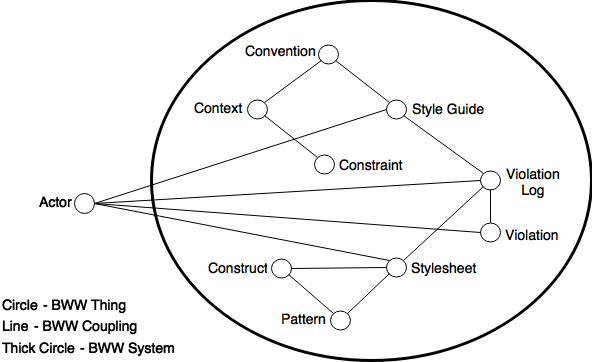
\includegraphics[width=0.8\textwidth]{ontology}
\end{figure}

According to the theory, a coupling occurs when the existence of a given thing affects the history of another thing and, in turn, history is defined as the chronological ordered states that a thing traverses~\cite{wand1990ontological}. Thus, in the domain-specific ontology a coupling exist between the Style Guide and the Convention things, because the existence of a Convention alters the state of the Style Guide. Similarly, a Context changes the state of a Convention and a Constraint affects the state of a Context. 

There are also couplings between Construct, Pattern and Stylesheet things. Both Stylesheet and Pattern are composed of Constructs, and thus affected by their existence. Since a Pattern is a specific occurrence of a combination of Constructs, it is also coupled to Stylesheet.

A Violation is coupled to a Violation Log, since the presence of a new a Violation alters the state of the log. Further, a Violation Log contains information about the violations of a particular Style Guide that occur in a specific Stylesheet. In this sense, a Violation Log is a function of a Style Guide and a Stylesheet and it is coupled to both things.

There are two external events that an Actor can initiate: searching for violations and discovering violations. Both of these events express couplings, because they change the state of the Violation Log and the Violation, respectively. Note that an Actor can create any of the things that appear in Figure 5.1. In practice, the Actor can introduce additional Conventions, change the Style Guide, alter the existing Constructs and rewrite the Stylesheet. However, these events are considered outside the domain of the designed ontology. 

\subsection{Ontological analysis}

\textbf{Representation Mapping}

\begin{center}
\begin{longtable}{ | p{17em} | p{23em} | } 
\caption{Representation mapping}\\
\hline
 &  \\
Ontological concepts & Semantic constructs \\
 &  \\
\hline
Style Guide & Convention Set \\ \hline
Number of Conventions of Style Guide & Conventions of Convention Set \\ \hline
Convention & Convention \\ \hline
Description of Convention  & Description of Convention \\ \hline
Exception of Conventions & Exceptions of Convention \\ \hline
Allowance of Conventions & Relaxing Conventions of Convention \\ \hline
Context & Pattern descriptor, Node descriptor, Node Relation \\ \hline
Ignored Constructs & Convention Context \\ \hline
Constraint & Expression \\ \hline
Subject of Constraint & API Call, Literal Expression, Variable Expression \\ \hline
Comparison Constraint & Comparison Expression \\ \hline
Type Constraint & Is Expression \\ \hline
Textual Form Constraint & Match Expression \\ \hline
Set Membership Constraint & Set Membership Expression \\ \hline
Context Constraint & Context Query Expression \\ \hline
Violation Log & Violation Log \\ \hline
Number of Violations & Violations of Violation Log \\ \hline
Violation & Violation \\ \hline
Description of Violation & Description of Violation \\ \hline
Position in Stylesheet of Violation & Position of Violation \\ \hline
Stylesheet & Tree \\ \hline
Construct & Node \\ \hline
Type of Construct & Search Categories of Node \\ \hline
Textual Representation of Construct & String of Node \\ \hline
CSS-specific knowledge & API of Node \\ \hline
Relation between Constructs & Node Relation \\ \hline
Pattern & Node, Node Relation \\ \hline
Number of Constructs of Pattern & Node Descriptors of Pattern Descriptor \\ \hline
\end{longtable}
\end{center}


\begin{center}
\begin{longtable}{ | p{23em} | p{17em} | } 
\caption{Interpretation mapping}\\
\hline
 &  \\
Semantic constructs & Ontological concepts  \\
 &  \\
\hline

Convention Set & Style Guide \\ \hline
Conventions of Convention Set & Number of Conventions of Style Guide \\ \hline
Convention Context & Ignored Constructs of a Context \\ \hline
Convention & Convention \\ \hline
Description property of Convention & Description of Convention \\ \hline
Exceptions of Convention & Exception of Conventions \\ \hline
Relaxing Conventions of Convention & Allowance of Conventions \\ \hline
Pattern Descriptor, Node Descriptor, Node Relation & Context \\ \hline
Node Descriptors of Pattern Descriptor & Number of Constructs of Pattern \\ \hline
Expression, Logical Expression & Constraint \\ \hline
Comparison Expression & Comparison Constraint \\ \hline
Is Expression & Type Constraint \\ \hline
Match Expression  & Textual Form Constraint \\ \hline
Set Membership Expression & Set Membership Constraint \\ \hline
Context Query Expression & Context Constraint \\ \hline
API Call, Literal Expression, Variable Expression & Constraint Subject \\ \hline
Node & Construct \\ \hline
Search Categories of Node & Type of Construct \\ \hline
String of Node & Textual Representation of Construct \\ \hline
API of Node & CSS-specific knowledge of Construct \\ \hline
Node, Node Relation & Pattern \\ \hline
Tree & Stylesheet \\ \hline
Violations Log & Violations Log \\ \hline
Violations of Violations Log & Number of Violations \\ \hline
Violation & Violation \\ \hline
Description of Violation & Description of Violation \\ \hline
Position of Violation & Position in Stylesheet of Violation \\ \hline
\end{longtable}
\end{center}

%%%%%%%%%%%%%%%%%%%%%%%%%%%%%%%%%%%%%%%%%%%%%%%%%%%%%%%%%%%%%%%%%%%%%%%%%%%%%%%

\chapter{Conclusion}

This work makes several contributions. 1) 2) It contains a summary of existing
CSS coding conventions. 3) It designs a domain specific language that expresses
conventions and its interpreter to detect violations automatically.

{%\tiny
\bibliographystyle{alphaurl}
\bibliography{thesis}
}

\end{document}
